\section{M-SPLearning Experimental Evaluation}\label{section4}


This section presents the experimental evaluation of M-SPLearning with respect to time-to-market and quality improvement. M-SPlearning was compared with software singular development methodology. The guidelines proposed by Jedlitschka et al. \cite{jedlitschka07} were followed to report controlled experiments.

\subsection{Motivation}\label{sub:motivation}


The choice in the adoption of new technologies or approaches used in development process depends on which aspects of quality and benefits are desired. Despite the fact of many approaches have been established in the literature, there are many issues to be solved about them to conduct a suitable adoption in both industry and academic environments. Experimental evaluations may bring the light in the identification of evidences from quality aspects and benefits in these approaches, supporting the choice of them. In some cases, the collected evidence may still supports the correction of problems identified during the experimental evaluations, allowing the improvement of the proposals.

Therefore, to collect initial evidence in two crucial development perspectives, time-to-market and quality in terms of number of faults, the experimental evaluation of the M-SPlearning is presented.

In the context of the experiment conducted, time-to-market is the average time spent for the implementation of a software product with a specific group of variabilities of M-SPLearning. With regard to the number of faults, the implemented products were tested using the concept of test cases \cite{craig02}. Thus, it was possible to quantify the mean of defects of products. Such metrics are relevant because they are directly related to time-to-market and quality of the m-learning applications.


%\subsubsection{Problem Statement}


\subsubsection{Research Objectives}\label{sub:object}

The goal of the experiment was to \textbf{compare} the singular software development methodology (SSD) and the software product line (SPL) methodology, \textbf{for the purpose of} identifying the most efficient, \textbf{with respect to} the time spent for creating software products (time) and the number of faults of the created software products, \textbf{in the context of} practitioners from industry.


%\subsubsection{Context}

%\subsection{Related Work}\label{sub:rel_work}


\subsection{Experimental Design}\label{sub:design}

This section provides the experimental design and procedures for supporting future replications.


\subsubsection{Goals}

Based on the research objective two research questions (R.Q.) were stated:


\textbf{R.Q.1} Which methodology is more efficient with respect to time-to-market, SSD or SPL?

\textbf{R.Q.2} Which methodology showed more quality in terms of the number of faults in the created software product, SSD or SPL?

\subsubsection{Hypotheses}

Two sets of hypotheses were defined to be tested, each of them related with its respective research questions (R.Q.1 and R.Q.2):


\textbf{R.Q.1 hypotheses:} time-to-market

	\begin{itemize}
	
	\item \textbf{Null Hypothesis ($H_{0}$)}: there is no significant of time-to-market between SSD and SPL.
	
	$H_{0}$ : $\mu$(\textit{t(SSD)}) =  $\mu$(\textit{t(SPL)});
	
	
	\item \textbf{Alternative Hypothesis ($H_{1}$)}: SSD has less time-to-market than SPL.
	
	$H_{1}$ : $\mu$(\textit{t(SSD)}) $<$ $\mu$(\textit{t(SPL)});
		
	
	\item \textbf{Alternative Hypothesis ($H_{2}$)}: SSD has more time-to-market than SPL.
	
	$H_{2}$ :  $\mu$(\textit{t(SSD)}) $>$ $\mu$(\textit{t(SPL)}).		
	
	\end{itemize}	



\textbf{R.Q.2 hypotheses:}
quality in terms of the number of faults
	\begin{itemize}
	
	\item \textbf{Null Hypothesis ($H_{0}$)}: there is no significant difference between SSD and SPL with regard to quality in terms of number of faults in the software products created.
	
	$H_{0}$ : $\mu$(\textit{d(SSD)}) =  $\mu$(\textit{d(SPL)});
	
	
	\item \textbf{Alternative Hypothesis ($H_{1}$)}: SSD has greater number of faults than SPL.
	
	$H_{1}$ : $\mu$(\textit{d(SSD)}) $>$ $\mu$(\textit{d(SPL)});
		
	
	\item \textbf{Alternative Hypothesis ($H_{2}$)}: SSD has minor number of faults than SPL.
	
	$H_{2}$ :  $\mu$(\textit{d(SSD)}) $<$ $\mu$(\textit{d(SPL)}).		
	
	\end{itemize}


\subsubsection{Variables}

Dependent variables are the mean of time ($t$) and faults ($f$), defined as follows:

\small

\begin{equation}\label{eq:1}
\mu{(t)}=(\Sigma xi)/n, i = 1..n
\end{equation}
\begin{equation}\label{eq:2}
\mu{(f)}=(\Sigma yi)/n, i = 1..n
\end{equation}
\normalsize 
where:
\begin{itemize}
\item \textit{t} is the time of implementation (minutes);
\item \textit{f} is the number of faults;
\item \textit{xi} is the time of implementation of subject i;
\item \textit{yi} is the number of faults detected in the implementation of subject i; and
\item \textit{n} is the total of subjects in the experiment.
\end{itemize}
\normalsize

Independent variables are the development methodology, which is a factor with two treatments (SSD and SPL) and the software product configuration for mobile learning platform, which is a factor with two treatments: product 1 (P1) and product 2 (P2). Table \ref{tab:variables} presents the description of dependent and independent variables.


\begin{landscape}
\centering
\begin{table}[h]
\caption{\label{tab:variables}Dependent and Independent Variables Description.}
\resizebox{1.4\textwidth}{!}{
\small
\begin{tabular}{cccccccccc}
\multicolumn{1}{l}{}                                                                         & \multicolumn{1}{l}{}                                                                                                                      & \multicolumn{1}{l}{}                                 & \multicolumn{1}{l}{}                                                                                                        & \multicolumn{1}{l}{}                                                                                           & \multicolumn{1}{l}{}                                                                                                        & \multicolumn{1}{l}{}                                                                                            & \multicolumn{1}{l}{}                                                                & \multicolumn{1}{l}{}                                                                                                                             & \multicolumn{1}{l}{}                                              \\ \hline
\multicolumn{1}{c|}{\textbf{\begin{tabular}[c]{@{}c@{}}Name of the\\ Variable\end{tabular}}} & \multicolumn{1}{c|}{\textbf{\begin{tabular}[c]{@{}c@{}}Type of the\\ Variable\\ (independent, \\ dependent, \\ moderating)\end{tabular}}} & \multicolumn{1}{c|}{\textbf{Abbreviation}}           & \multicolumn{1}{c|}{\textbf{\begin{tabular}[c]{@{}c@{}}Class\\ (product, \\ process, \\ resource, \\ method)\end{tabular}}} & \multicolumn{1}{c|}{\textbf{\begin{tabular}[c]{@{}c@{}}Entity\\ (instance of \\ the class)\end{tabular}}}      & \multicolumn{1}{c|}{\textbf{\begin{tabular}[c]{@{}c@{}}Type of \\ Attribute \\ (internal, \\ external, \ \ldots)\end{tabular}}} & \multicolumn{1}{c|}{\textbf{\begin{tabular}[c]{@{}c@{}}Scale\\  Type \\ (nominal, \\ ordinal,\ \ldots)\end{tabular}}} & \multicolumn{1}{c|}{\textbf{Unit}}                                                  & \multicolumn{1}{c|}{\textbf{Range}}                                                                                                              & \textbf{\begin{tabular}[c]{@{}c@{}}Counting \\ Rule\end{tabular}} \\ \hline
\multicolumn{1}{c|}{\begin{tabular}[c]{@{}c@{}}Development\\ methodology\end{tabular}}       & \multicolumn{1}{c|}{\multirow{2}{*}{independent}}                                                                                         & \multicolumn{1}{c|}{DM}                              & \multicolumn{1}{c|}{method}                                                                                                 & \multicolumn{1}{c|}{\begin{tabular}[c]{@{}c@{}}Software\\ development \\ methodology\end{tabular}}             & \multicolumn{1}{c|}{N.A.}                                                                                                   & \multicolumn{1}{c|}{nominal}                                                                                    & \multicolumn{1}{c|}{N.A.}                                                           & \multicolumn{1}{c|}{\begin{tabular}[c]{@{}c@{}}SSD – Singular \\ software \\ development \\ and SPL – Software \\ product\\  line.\end{tabular}} & N.A.                                                              \\ \cline{1-1} \cline{3-10} 
\multicolumn{1}{c|}{\begin{tabular}[c]{@{}c@{}}Software\\ Products\end{tabular}}             & \multicolumn{1}{c|}{}                                                                                                                     & \multicolumn{1}{c|}{P}                               & \multicolumn{1}{c|}{product}                                                                                                & \multicolumn{1}{c|}{\begin{tabular}[c]{@{}c@{}}Mobile\\ Software \\ Product\end{tabular}}                      & \multicolumn{1}{c|}{N.A.}                                                                                                   & \multicolumn{1}{c|}{nominal}                                                                                    & \multicolumn{1}{c|}{N.A.}                                                           & \multicolumn{1}{c|}{P1 and P2.}                                                                                                                  & N.A.                                                              \\ \hline
\multicolumn{10}{c}{}                                                                                                                                                                                                                                                                                                                                                                                                                                                                                                                                                                                                                                                                                                                                                                                                                                                                                                                                                                                                                                                                                       \\ \hline
\multicolumn{1}{c|}{\begin{tabular}[c]{@{}c@{}}Time of \\ implementation\end{tabular}}       & \multicolumn{1}{c|}{\multirow{2}{*}{dependent}}                                                                                           & \multicolumn{1}{c|}{\begin{equation}t\end{equation}} & \multicolumn{1}{c|}{product}                                                                                                & \multicolumn{1}{c|}{\begin{tabular}[c]{@{}c@{}}time to\\ market\end{tabular}}                                  & \multicolumn{1}{c|}{\begin{tabular}[c]{@{}c@{}}internal: time;\\  external: time to \\ market\end{tabular}}                 & \multicolumn{1}{c|}{ordinal}                                                                                    & \multicolumn{1}{c|}{Minutes} & \multicolumn{1}{c|}{\begin{tabular}[c]{@{}c@{}}From 00:00:00 to \\03:00:00.\end{tabular}}                                                                                                                   & \begin{tabular}[c]{@{}c@{}}Eq. 1\end{tabular}           \\ \cline{1-1} \cline{3-10} 
\multicolumn{1}{c|}{Faults}                                                                  & \multicolumn{1}{c|}{}                                                                                                                     & \multicolumn{1}{c|}{\begin{equation}f\end{equation}} & \multicolumn{1}{c|}{product}                                                                                                & \multicolumn{1}{c|}{\begin{tabular}[c]{@{}c@{}}number of\\ faults in\\ each\\ software\\ product\end{tabular}} & \multicolumn{1}{c|}{\begin{tabular}[c]{@{}c@{}}internal: faults;\\ external: quality\end{tabular}}                          & \multicolumn{1}{c|}{ordinal}                                                                                    & \multicolumn{1}{c|}{Integer} & \multicolumn{1}{c|}{any integer}                                                                                                                 & \begin{tabular}[c]{@{}c@{}}Eq. 2\end{tabular}           \\ \hline

\end{tabular}
}
\end{table}
\end{landscape}

%\subsubsection{Experiment Design}

\subsubsection{Subjects}

%Despite the fact that evaluations executed in academic laboratories are important to bring light about the study object, the conduction only in this controlled environments and with toys examples makes the evidence questionable in some cases \cite{wohlin12}. 

In our study, the subjects were practitioners volunteers from a Brazilian software development industry. All of them had, at least, one year of experience, with development background in Java, Microsoft .NET and/or PHP.

The reduced number of practitioners led us to apply a non-random selection. The random capacity was applied at the assignment of the development methodology and the software product to each participant. 

Block classification was defined by the two factors with two treatments, which were interspersed in four set of documents. Thus, the population was divided into four blocks by means of a draw. The balancing was applied in the tasks, that were assigned in equal numbers to a similar number of subjects.

Participants were randomly separated into the following groups:

\begin{itemize}
\item \textbf{First Group:} focused in SSD with P1, them in SPL with P2;

\item \textbf{Second Group:} focused in SPL with P1, and in SSD with P2;

\item \textbf{Third Group:} focused in SSD with P2, and with SPL with P1; and

\item \textbf{Fourth Group:} focused in SPL with the P2, and with SSD with P1;
\end{itemize}


\subsubsection{Objects}

Among a total of 30 features and diferent configurations, two educational software products configurations for mobile learning platform (Android) were taken into consideration to apply the SSD and SPL methodologies which are: one for image (P1) and another for video resource (P2).

\subsubsection{Instrumentation}

The experiment was supported by a set of instruments: (i) similar desktop computers with all necessary tools (Eclipse IDE and plugins); (ii) the consent term to the experimental study; (iii) a characterization questionnaire; (iv) use case, component and sequence UML diagrams; (v) interface messages; (vi) database model; (vii) one project base; (viii) composed of the similarities of the products; (ix) the experimental forms for SSD and SPL, randomly distributed and feedback questionnaire.

\subsubsection{Data Collection and Analysis Procedure}

%The main assessment tools were the software products specifications (P1 and P2) for mobile learning platform (Android), to allow the development of the product, distributed in an equal number.


The main assessment tools were the products developed based in two software specifications (P1 and P2) for mobile learning platform (Android).

Based on the catalog of requirements (Section \ref{section2}), the M-SPLearning was designed with a total of 30 features from m-learning applications having 16 mandatory features and 14 optional features. A specific niche of features was used for our experimental evaluation, where the variabilities related to multimedia resources let one to create up to 15 different products (as represented by Figure \ref{figureMSPLFeatureModel}). Two specifics products (P1 and P2) were specified and implemented using both SSD and SPL methodologies. Figure \ref{fig:prod} represents the nuances between products generated for the video feature.


\begin{figure*}[t]
\centering
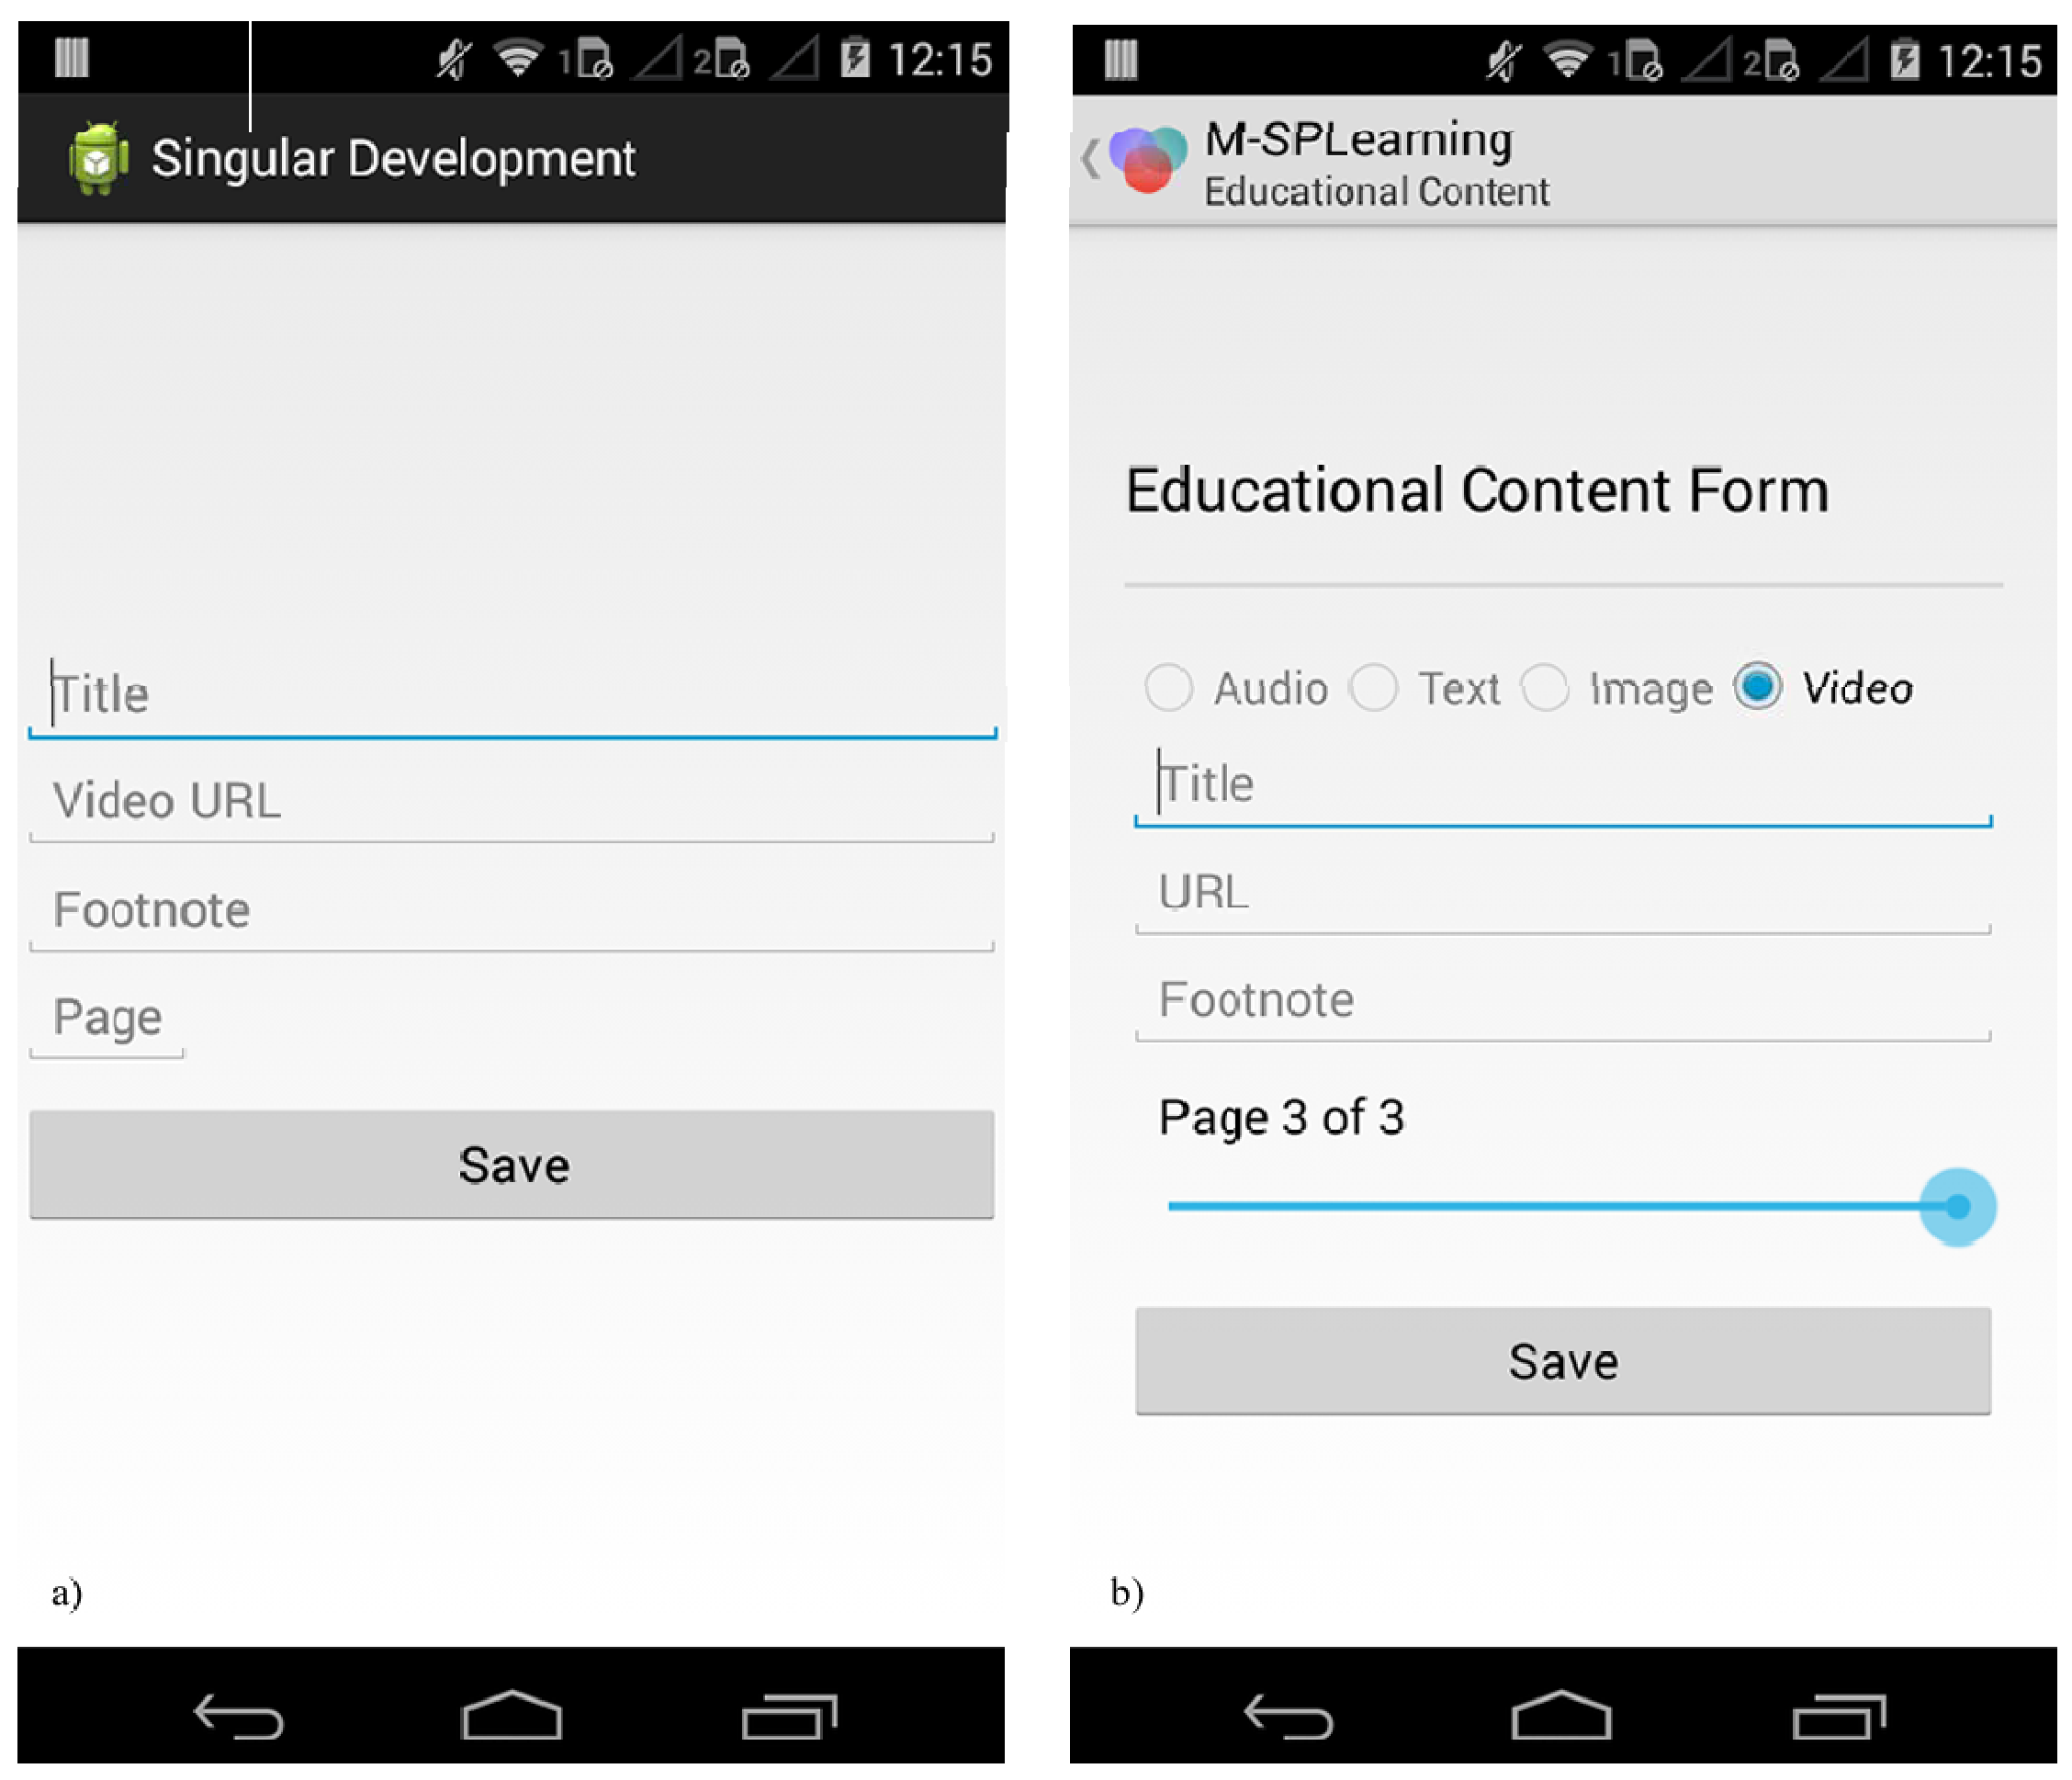
\includegraphics[scale=0.2]{figures/section4/prod.eps}
\centering
\caption{Two Video Products (P1) Developed in the Experimental Execution with a) SDD and b) SPL.}
\label{fig:prod}
\end{figure*}


To collect the data for the analysis of time-to-market, the initial and final time of implementation process for P1 and P2, was registered individually in the experimental form to be calculated in Equation \ref{eq:1}. On the other hand, for the analysis of quality, each of 15 finished developed products were tested and the number of faults was collect to compare the use of SPL and SDD methodologies by means of the Equation \ref{eq:2}.


\subsubsection{Validity Evaluation}

A pilot project was conducted with two pratictioners from industry, evaluating the study instrumentation and allowing to estimate the duration of the training and execution sessions. The pilot results, such as the subjects were not used in the final execution and data analysis of the experiment.


\subsection{Execution}\label{sub:execution}

This section presents how the experimental plan (design) was enacted.

\subsubsection{Sample}

The sample was composed of a total of 21 pratictioners who participated in the training session. However, 18 subjects participated in the experimental execution, due the unavailability of 3 volunteers in the execution day.

\subsubsection{Preparation}

The subjects were trained with regard to essential concepts of Android development for SSD and SPL with the Eclipse IDE. The training lasted three days. The knowledge of the subjects was evaluated with essays in the end of each training session. In the fourth day, the experiment was performed.

\subsubsection{Data Collection Performed}

The procedures adopted for data collection were:

\begin{enumerate}

\item the subjects participated in three trainning sessions, one per day, lasting 4 hours, in industrial environment;
%\item in the fourth day the subject came along the place where the study was conducted, the same were the training sessions were conducted;
\item the subjects were divided in four groups by means of a draw;
\item the experimenter gave the subject a set of documents: the UML diagram models, dataset model, interface message specification for each product, such as the material used in training session. Each one was allocated in a desktop computer, with all requirements to develop the software product. Besides, each subject received an experimental form where they registered the spending time to development process to be analysed.
\item the subject reads each given document;
\item the experimenter explains the given documents;
\item the subject reads and clarifies possible doubts about the products specifications; and
\item finally, each subject received and used two randomly drawn methodologies to development a requested m-learning product. They were warning that they must applied each methodology following the receive order. Besides, for each application, subjects registered the lasting of the application (start time, end and brakes). In the end of the two development tasks for the two methodologies they were invited to answer an feedback questionnaire. In this questionnaire, subjects gave their opinion about the experimental execution and the used technologies.
\end{enumerate}





%\subsubsection{Validity Procedure}




\subsection{Analysis}\label{sub:analysis}

As the experiment session was finished, collected data was prepared (tabulation and descriptive statistics) to be applied in statistical tests.

\subsubsection{Collected Data and Descriptive Statistics}

For each subject (``\texttt{Subject \#}'' column), we collected the following data: the total time of implementation and the total number of faults, identified by testing procedures, and the mean calculation. Those results are presented in Table \ref{tab:resul1}. The results for each subject was plotted in box-plots in Figure \ref{fig:boxplot}. 


\begin{table}[!ht]
\caption{\label{tab:resul1}SSD and SPL Collected Data and Descriptive Statistics.}
    \centering
    \scriptsize
\begin{tabular}{c|c|c|c|c}
\hline
\multirow{2}{*}{\textbf{Subject \#}} & \multicolumn{2}{c|}{\textbf{SSD}} & \multicolumn{2}{c}{\textbf{SPL}}  \\ \cline{2-5}
                                    & \textbf{Time $(t)$}   & \textbf{Faults $(f)$} & \textbf{Time $(t)$}  & \textbf{Faults $(f)$}                                  \\ \hline
1                                   & 161             & 15              & 2              & 9                                              \\ \hline
2                                   & 90              & 8               & 1              & 0                                             \\ \hline
3                                   & 105             & 4               & 11             & 0                                              \\ \hline
4                                   & 104             & 1               & 3              & 0                                             \\ \hline
5                                   & 73              & 2               & 1              & 0                                             \\ \hline
6                                   & 99              & 9               & 3              & 0                                              \\ \hline
7                                   & 165             & 12              & 10             & 0                                              \\ \hline
8                                   & 95              & 1               & 3              & 0                                              \\ \hline
9                                   & 104             & 3               & 2              & 0                                               \\ \hline
10                                  & 102             & 0               & 4              & 0                                              \\ \hline
11                                  & 61              & 0               & 2              & 0                                             \\ \hline
12                                  & 82              & 4               & 8              & 0                                              \\ \hline
13                                  & 114             & 1               & 4              & 0                                             \\ \hline
14                                  & 103             & 6               & 14             & 0                                            \\ \hline
15                                  & 111             & 2               & 2              & 0                                              \\ \hline
16                                  & 176             & 9               & 4              & 0                                              \\ \hline
17                                  & 120             & 17              & 5              & 0                                             \\ \hline
18                                  & 175             & 34              & 2              & 9                                              \\ \hline
\textbf{Mean}                       & \textbf{113.33} & \textbf{7.11}   & \textbf{4.50}  & \textbf{1.00}                 \\ \cline{1-5}
\textbf{Median}                     & \textbf{104}    & \textbf{4}      & \textbf{3}     & \textbf{0}                                      \\ \cline{1-5}
\textbf{Std. Dev.}                  & \textbf{33.98}  & \textbf{8.46}   & \textbf{3.75}  & \textbf{2.91}                             \\ \hline
\end{tabular}
\end{table}


\begin{figure}[!ht]
\centering
\includegraphics[scale=1.0]{./figures/section4/boxplot.eps}
\centering
\caption{Collected Data Box-Plot from SSD and SPL faults and SSD and SPL time-to-market.}
\label{fig:boxplot}
\end{figure}

%\subsubsection{Data Set Reduction}

\subsubsection{Hypothesis Testing}

%Based on the results obtained by analyzing the use of SSD and SPL to the development of two mobile learning products, the following steps were taken for answering the study research questions and testing the hypotheses:


%\begin{itemize}
%\item analyze and interpret the SSD and SPL collected data (Table \ref{tab:resul1} and Figure \ref{fig:boxplot}) by means of the Shapiro-Wilk normality test and the %Mann-Whitney-Wilcoxon hypothesis test, to validate their statistical power and compare them.
%\end{itemize}

Based on the results obtained by the use of SSD and SPL to the development of two mobile learning products, we summarize, analyze and interpret the SSD and SPL collected data (Table \ref{tab:resul1} and Figure \ref{fig:boxplot}) by means of the Shapiro-Wilk normality test and the Mann-Whitney-Wilcoxon hypothesis test. Both of them were used to validated the statistical power of the sample, allowing test the hypotheses.





\subsubsection{Efficiency in the Time of Implementation (R.Q.1)}
%ajustar o titulo desta seção


\begin{itemize}

%(Table \ref{tab:resul1})
\item \textbf{Collected Data Normality Tests:} the Shapiro-Wilk \cite{shaphirowilk65} normality test was applied to SSD and SPL time and faults, providing the following results:\\

\textbf{\textit{SSD time (\textit{N}=18):}}

For a mean value ($\mu$) 113.33, standard deviation value of ($\sigma$) 33.98, the time for the SSD was \textit{p} = 0.0274.

In the \textit{Shapiro-Wilk} test for a sample size \textit{(N)} 18 with 95\% of significance level ($\alpha$ = 0.05), \textit{p} = 0.0274 (0.0274 $<$ 0.05) and calculated value of \textit{W} = 0.8813 $<$ \textit{W} = 0.8970, the sample is considered non-normal.

%\textbf{\textit{SSD faults (\textit{N}=18):}}
%
%For a mean value ($\mu$) 7.11, standard deviation value of ($\sigma$) 4, the faults for the SSD was \textit{p} = 0.0006 for the \textit{Shapiro-Wilk} normality test.
%
%For a sample size \textit{(N)} 18 with 95\% of significance level ($\alpha$ = 0.05), \textit{p} = 0.0006 (0.0006 $<$ 0.05) and calculated value of \textit{W} = 0.7740 $<$ \textit{W} = 0.8970, the sample is considered non-normal.




\textbf{\textit{SPL time (\textit{N}=18):}}

For a mean value ($\mu$) 4.50, standard deviation value of ($\sigma$) 3.75, the time for the SPL was \textit{p} = 0.0014.

For a sample size \textit{(N)} 18 with 95\% of significance level ($\alpha$ = 0.05), \textit{p} = 0.0014 (0.0014 $<$ 0.05) and calculated value of \textit{W} = 0.7978 $<$ \textit{W} = 0.8970, the sample is considered non-normal.

%\textbf{\textit{SPL faults (\textit{N}=18):}}
%
%For a mean value ($\mu$) 1.00, standard deviation value of ($\sigma$) 0, the faults for the SPL was \textit{p} = 0.00000007 for the \textit{Shapiro-Wilk} normality test.
%
%For a sample size \textit{(N)} 18 with 95\% of significance level ($\alpha$ = 0.05), \textit{p} = 0.00000007 (0.00000007 $<$ 0.05) and calculated value of \textit{W} = 0.3730 $<$ \textit{W} = 0.8970, the sample is considered non-normal.





%\item \textbf{Mann-Whitney-Wilcoxon for SSD and SPL time samples:} this kind of test can be applied for both independent and paired samples. In the case of this study, SSD and SPL samples are independent and both samples are non-normal, thus it was defined the following hypothesis:


%\begin{itemize}
%  \item \textbf{Null Hypothesis ($H_{0}$)}: SSD took the same time of SPL, to implement a product.	
	
%	$H_{0}$ : $\mu$(\textit{t(SSD)}) = $\mu$(\textit{t(SPL)}); 
	
%	\item \textbf{Alternative  Hypothesis ($H_{1}$)}: SSD and SPL has different time of implementation.	
	
%	$H_{1}$ :  $\mu$(\textit{t(SSD)}) $<>$ $\mu$(\textit{t(SPL)}).

%	\end{itemize}	

\item \textbf{Mann-Whitney-Wilcoxon for SSD and SPL time samples:} a rank with weights were assigned for each sample value. The weights were added and applied in Equation \ref{eq:MWW}:
\small
\begin{equation}
\begin{split}
\label{eq:MWW}
U(DM) = N_1 * N_2 + \frac{N_1*(N_1+1)}{2} - \sum_{i=1}^{n} total_{2}
\end{split}
\end{equation}
\normalsize 
Where:
\begin{itemize}
\item \textit{$U(DM)$} is the equation for each of the independent sample (DM);
\item \textit{$N_1$} is the size of the sample for the X methodology that will be calculated;
\item \textit{$N_2$} is the size of the sample for the compared methodology (Y); and
\item \textit{$total_{2}$} is the sum of the weight given for the compared methodology.
\end{itemize}

For SSD the time value calculated with the Equation \ref{eq:MWW} was 326.5 and for SPL, the time value was 0.00.

%Equations \ref{eq:MWWP} and \ref{eq:MWWS} present the values for X and Y approaches, respectively.
%\small
%\begin{equation}
%\begin{split}
%\label{eq:MWWP}
%U(X) = 10 * 10 +  \frac{10 * (10+1)}{2} - 41 = 69.5
%\end{split}
%\end{equation}
%\normalsize 
%\small
%\begin{equation}
%\begin{split}
%\label{eq:MWWS}
%U(Y) = 10 * 10 + \frac{ 10 * (10+1)}{2} - 85.5 = 114
%\end{split}
%\end{equation}
%\normalsize 


%After calculating the equation for each approach, Equation \ref{eq:MWWT} is calculated:
%\small
%\begin{equation}
%\begin{split}
%\label{eq:MWWT}
%U = min(U(SSD),U(SPL))
%\end{split}
%\end{equation}
%\normalsize 
%Where:
%\begin{itemize}
%\item \textit{$U$} is the value for the statistic test, which accepts or rejects the null hypothesis ($H_0$);
%\item \textit{$min(U(SSD),U(SPL))$} returns the smallest value obtained based in Equation \ref{eq:MWW}.
%\end{itemize}

%Equation \ref{eq:MWWT} indicates a statistical difference among the methodologies.

%With the value of $U=0$, which corresponds to the SSD, we conclude that there are significant differences which leads to reject the null hypothesis ($H_0$) and accepted the alternative hypothesis ($H_{1}$), where the SSD time is different from the SPL.


%The statistical test identifies if the two samples have the same distribution of their weights. 

Each weight matches with subject's development process time with SSD or SPL methodology. There are evidences that both values are differents ($326.5>0$), which leads to reject the null ($H_0$) hypothesis and accepted the alternative hypothesis ($H_{1}$).

Therefore, the answer for R.Q.1 was obtained: it means that the SSD is more efficient than the SPL to implement software products for mobile platform. The project base and the SPL used in the experiment need to be considered.


The subjects received the base project of the two software products to be developed using SSD or SPL. The projects base consists by similarities of the products and were developed to reduce the experimental execution duration. They were implemented in 480 minutes (8 hours).

If we consider the time lasting for the implementation of each project base, plus the total of development time to each subjects (480 minutes), the total time would be of 10680 minutes or 178 hours ($total_{time}$((subje\allowbreak cts(18) x minutes(480)) + 2040 = 10680 minutes). Taking into account the base project of the software product line, the time lasting by the 18 subjects was 81 minutes (1 hour and 35 minutes) and the total time would be 11361 minutes or 189 hours and 35 minutes ($total_{time}$((subjects(18) x minutes(4.5)) + 10599 = 11361 minutes). 

Comparing both values, the SPL development used 621 minutes (11 hours and 35 minutes) more than with SSD. However, after the SPL implementation, the line allows the evolution and insertion of new variabilities, guaranteeing the faster generation of new products in addition to other advantages of the adoption of SPL approach.



\end{itemize}




\subsubsection{Number of faults of the created software products (R.Q.2)}
%ajustar o titulo desta seção


\begin{itemize}

%(Table \ref{tab:resul1})
\item \textbf{Collected Data Normality Tests:} 

\textbf{\textit{SSD faults (\textit{N}=18):}}

For a mean value ($\mu$) 7.11, standard deviation value of ($\sigma$) 4, the faults for the SSD was \textit{p} = 0.0006 for the \textit{Shapiro-Wilk} normality test.

For a sample size \textit{(N)} 18 with 95\% of significance level ($\alpha$ = 0.05), \textit{p} = 0.0006 (0.0006 $<$ 0.05) and calculated value of \textit{W} = 0.7740 $<$ \textit{W} = 0.8970, the sample is considered non-normal.



\textbf{\textit{SPL faults (\textit{N}=18):}}

For a mean value ($\mu$) 1.00, standard deviation value of ($\sigma$) 0, the faults for the SPL was \textit{p} = 0.00000007 for the \textit{Shapiro-Wilk} normality test.

For a sample size \textit{(N)} 18 with 95\% of significance level ($\alpha$ = 0.05), \textit{p} = 0.00000007 (0.00000007 $<$ 0.05) and calculated value of \textit{W} = 0.3730 $<$ \textit{W} = 0.8970, the sample is considered non-normal.





\item \textbf{Mann-Whitney-Wilcoxon for SSD and SPL faults samples:} it was defined the following hypothesis for the number of faults:


\begin{itemize}
  \item \textbf{Null Hypothesis ($H_{0}$)}: SSD had the same number of faults than SPL.	
	
	$H_{0}$ : $\mu$(\textit{t(SSD)}) = $\mu$(\textit{t(SPL)}); 
	
	\item \textbf{Alternative  Hypothesis ($H_{1}$)}: SSD and SPL had different number of faults.	
	
	$H_{1}$ :  $\mu$(\textit{t(SSD)}) $<>$ $\mu$(\textit{t(SPL)}).

	\end{itemize}	

For SSD the number of faults calculated with the Equation \ref{eq:MWW} was 282 and for SPL, the number of faults was 42.



%Equation \ref{eq:MWWT} indicates a statistical difference among the methodologies.







%With the value of $U=42$, which corresponds to the SSD, we conclude that there are significant differences which leads to reject the null hypothesis ($H_0$) and accepted the alternative hypothesis ($H_{1}$), where the SSD number of faults is different from the SPL.




%The statistical test identifies if the two samples have the same distribution of their weights. 

Each weight matches with subject's development project faults with SSD or SPL methodology. There are evidences that both values are differents ($282>42$), which leads to reject the null ($H_0$) hypothesis and accepted the alternative hypothesis ($H_{1}$).

Therefore, based on the result from the Mann-Whitney-Wilcoxon, the answer for R.Q.2 was obtained: it means that the SSD is prone to showed more faults in the software products developed than the SPL.




\end{itemize}







\subsection{Interpretation and Discussion}\label{sub:interpretation}

%\subsubsection{Evaluation of Results and Implications}
Data collected from SSD and SPL application was analyzed and interpreted. %, to validate their statistical power and compare them. The normality tests and statistical tests 
Results are summarized in Table \ref{tab:resul_s}.




\begin{table}[!ht]
\caption{\label{tab:resul_s}SSD and SPL Normality and Statistical Tests Results.}
\centering
\includegraphics[scale=0.96]{figures/section3/figtab.pdf}

%\scriptsize
%%\resizebox{0.87\textwidth}{!}{\begin{minipage}{\textwidth}
%\begin{tabular}{ccc}
%\hline
%\multicolumn{1}{c|}{\textbf{Element}}                                      & \multicolumn{1}{c|}{\textbf{SSD}}                          & \textbf{SPL}                                 \\ \hline
%\multicolumn{1}{c|}{\multirow{2}{*}{\textbf{Selection of Subjects}}}       & \multicolumn{2}{c}{18 practitioners.}                                                                     \\ \cline{2-3} 
%\multicolumn{1}{c|}{}                                                      & \multicolumn{1}{c|}{N(SSD)=18}                             & N(SPL)=18                                    \\ \hline
%\multicolumn{3}{c}{\textbf{Time to Implementation}}                                                                                                                                            \\ \hline
%\multicolumn{1}{c|}{\textbf{Mean}}                                         & \multicolumn{1}{c|}{113.33}                                & 4.5                                          \\ \hline 
%\multicolumn{1}{c|}{\multirow{2}{*}{\textbf{Shapiro-Wilk Normality Test}}} & \multicolumn{1}{c|}{p = 0.0274 (0.0274 \textless 0.05)}    & p = 0.0014 (0.0014 \textless 0.05)           \\
%\multicolumn{1}{c|}{}                                                      & \multicolumn{1}{c|}{Non-normal.}                           & Non-normal.                                  \\ \hline
%\multicolumn{1}{c|}{\multirow{2}{*}{\textbf{Statistical Test}}}            & \multicolumn{2}{c}{Mann-Whitney-Wilcoxon}                                                                 \\
%\multicolumn{1}{c|}{}                                                      & \multicolumn{2}{c}{(326.5 \textgreater 0) Evidence of statistical differences among times.}            \\ \hline
%\multicolumn{1}{c|}{\textbf{Result}}                                       & \multicolumn{2}{c}{R.Q.1 $H_1$: SPL has less time-to-market than SSD.}                                                      \\ \hline
%\multicolumn{3}{c}{\textbf{Number of Faults}}                                                                                                                                \\ \hline
%\multicolumn{1}{c|}{\textbf{Mean}}                                         & \multicolumn{1}{c|}{7.11}                                  & 1                                            \\ \hline
%\multicolumn{1}{c|}{\textbf{Shapiro-Wilk Normality Test}}                  & \multicolumn{1}{c|}{p = 0.0006 (0.0006 \textless 0.05)}    & p = 0.00000007 (0.00000007 \textless 0.05)   \\ \hline
%\multicolumn{1}{c|}{\multirow{2}{*}{\textbf{Statistical Test}}}            & \multicolumn{2}{c}{Mann-Whitney-Wilcoxon}                                                                 \\
%\multicolumn{1}{c|}{}                                                      & \multicolumn{2}{c}{(282 \textgreater 42) Evidence of statistical differences among number of faults.} \\ \hline
%\multicolumn{1}{c|}{\textbf{Result}}                                       & \multicolumn{2}{c}{R.Q.2 $H_1$: SPL has less number of faults in the products than SSD.}                                    
%\end{tabular}
%%\end{minipage}}
\end{table}

In terms of time-to-market, the statistical difference showed by Mann-Whitney-Wilcoxon test provides evidence that SPL (i.e., M-SPLearning) was more efficient than SSD in the development of P1 and P2 m-learning products, thus answering R.Q.1. % similar products).

With regard to the number of faults, the statistical difference showed by Mann-Whitney-Wilcoxon test provides evidence that SSD showed more faults than SPL in the development of P1 and P2 m-learning products, thus answering R.Q.2. % similar products).

From the results of the Mann-Whitney-Wilcoxon test, both R.Q.1 and R.Q.2 null hypotheses can be rejected.

%\subsubsection{Limitations of the Study}
%\subsubsection{Inferences}
%\subsubsection{Lessons Learned}


\subsubsection{Threats to Validity}\label{sec:threats}

This section presents the actions taken to act directly against threats of thid experiment, according to the Conceptual Model of Anderlin Neto and Conte \cite{neto13}.

\textbf{Internal Validity:} %the following issues were considered:

\begin{itemize}
\item \textbf{Differences among subjects:} as we took subjects with different experience levels, variations in the subjects' skills were reduced during the training sessions. The assessments realized in the end of each day of training allowed to evaluate the level of knowledge in the content used in the experimental execution, thus guaranteeing the reduction of variations in subject's skills.

\item \textbf{Fatigue effects:} on average, the experiment lasted 180 minutes. Thus, fatigue was considered not relevant since the subjects were able to leave the room for a quick break. Periods of absence were registered to be not added in the period of time registered to be analysed.

\item \textbf{Influence among subjects:} the subjects performed the experiment under supervision of a human observer to mitigate the possible influence of communication among them.

\item \textbf{Trainning Sessions:} the explanations in training sessions were given not only for the question, but for every participant. This action was taken to avoid possible biases, and allowed that every training member stayed abreast of the answer for all doubts.
\end{itemize}


\textbf{External Validity:} %the following threats were detected:

\begin{itemize}

\item \textbf{Instrumentation:} m-learning products and other instruments were tested in the pilot project, being considered significant to analyze time-to-market and number of faults.

\item \textbf{Subjects:} more experiments considering different metrics with industry practitioners must be conducted in order to identify other relevant factors related to the adoption of M-SPLearning.

\end{itemize}



\begin{itemize}

\item \textbf{Construction Validity:} independent variables were tested in the pilot project to guarantee their validity.


\item \textbf{Conclusion Validity:} since the number of subjects is reduced, mainly by the number of practitioners in the industry, the sample size must be increased in prospective replications of the experiment. The results of this study is considered indicators, and not conclusive, although, the lack of experimental executions in industrial environment, even with small samples are important for the evaluation of the time-to-market and quality for both SSD and SPL.



\end{itemize}



%
%
%\subsection{Conclusion and Future Work}\label{sub:conclusion_f_w}
%
%\subsubsection{Relation to Existing Evidence}
%
%\subsubsection{Impact}
%
%\subsubsection{Limitations}
%
%\subsubsection{Future Work}
%








































